\documentclass[12pt,a4paper]{article}
\usepackage{graphicx}
\usepackage{amsmath}
\usepackage{amsfonts}
\usepackage{amssymb}
\usepackage{graphicx}
\usepackage[left=2cm,right=2cm,top=2cm,bottom=2cm]{geometry}
\pagestyle{headings}
\title{Report 3}

\begin{document}

 1/ Why you chose your specific MPI implementation?
- OpenMPI is a readily available package in Ubuntu Packages => easy installation.

2/ How you design your MPI service. Figure.
- The system has a root process and a number of process that the user choose.
- The file system is one-to-many, user can send a different file to each child process.
- The root process check the user input to see whether the file is valid.
- The root process sends the title and the content of the file seperately to the child process using a for loop through each child.

3/ How you organize your system?

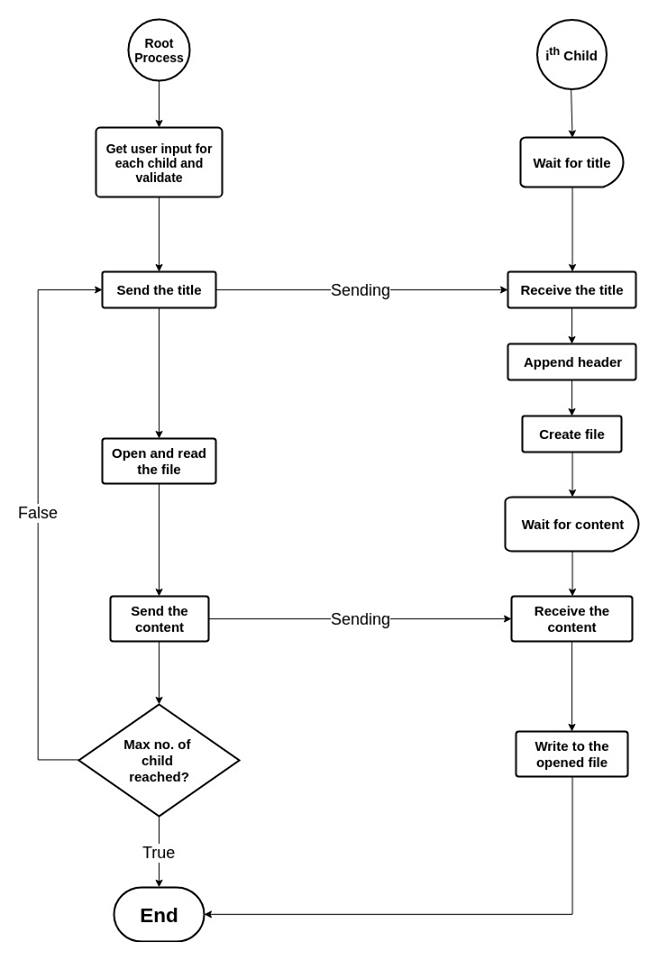
\includegraphics[scale=0.6]{mpi}
\end{document}


